\documentclass[sigconf,nonacm,article]{acmart}
\usepackage{array}

\setcopyright{none}

\begin{document}
\title{PDU Protocol: A Peer-to-Peer Social Netwrok Service}
\author{Peng Liu}
\email{liupeng@pdu.pub}

\begin{abstract}
   A fully peer-to-peer (P2P) social networking system should enable participants to freely publish and efficiently access information without relying on any third-party services. However, if the system does not employ centralized verification methods, such as phone numbers, allowing the cost-free creation of new accounts, it becomes susceptible to Sybil attacks. This vulnerability undermines the system’s reward and punishment mechanisms, inundates genuine content with spam, and renders the system unusable. This paper proposes a solution for constructing a P2P social network without relying on any third-party user authentication services. The scheme establishes a trusted publisher identity through a sequence of messages signed by the same private key. Interactions such as reposts, comments, and likes create associations between publishers. Based on these associations, participants can form a custom set of visible publisher identities. Within this relatively stable scope, an identity-based reward and punishment mechanism can be employed to effectively filter information.
\end{abstract}

\maketitle
\pagestyle{plain} % add page numbers, remove title/authors in the page header

\section{Introduction}\label{sec:introduction}

In today's online ecosystem, information dissemination and interaction primarily depend on centralized platforms like Facebook, Twitter/X, and WeChat. These platforms allow users to conveniently post information and establish connections, using various algorithms to detect and filter spam, thus ensuring user experience. However, the problems of centralized social services have become increasingly apparent. Third-party services may misuse user information or leak private data. They might leverage their extensive user base to lock in users and maintain their monopoly. Additionally, centralized services are prone to government regulation and censorship due to their clear and controllable targets.

Despite these issues, most users continue to rely on these existing platforms. While switching platforms does not result in data loss, it does lead to the loss of accumulated user relationships on the platform, thereby diminishing one's influence~\cite{Trust}. This lock-in effect significantly binds users to the platforms.

Decentralized social platforms have rapidly developed in recent years, attempting to address many issues posed by centralized platforms, exemplified by Mastodon. Mastodon employs a federated architecture~\cite{Mastodon}, eschewing a single center in favor of multiple intercommunicating servers, allowing users to retain control over their relationship data. However, the user registration process and content management still depend on server administrators. This governance structure can be seen as a collection of several small centralized platforms, failing to fundamentally avoid the issues faced by centralized platforms.

Blockchain-based social platforms like Steemit~\cite{Steemit}~\cite{SteemitModel} and Minds~\cite{Censorship} implement a certain number of tokens as the cost to create or activate accounts, while also incentivizing social behaviors with tokens. Although this approach increases the cost of account creation, it differs from the identity verification methods of centralized platforms. This method cannot effectively prevent the proliferation of fake accounts and imposes unfair restrictions on economically disadvantaged users, thus reducing the diversity and inclusiveness of the user base.

Some social software initially employs an invitation system to control the credibility of new users, effectively preventing malicious registrations and the spread of fake accounts. However, this approach also hinders the participation of a broader user base. For those who do not know existing users, joining the platform becomes exceedingly difficult. Moreover, early users significantly influence the community culture and rules, potentially leading to cultural homogeneity and difficulty in attracting a diverse user group.

This paper proposes a novel peer-to-peer social networking system that does not rely on any third-party services. Any sequence of messages signed with the same private key and possessing a total order is recognized by the system as a legitimate publisher identity, ensuring the immutability of information and providing a fair assessment of publisher identities. Through interactions among messages, public associations between publisher identities can be formed, viewed as trust relationships among users. Any user can maintain a visible set of publisher identities based on these associations, using custom rules, and within this scope, effectively filter information using publisher identities as markers.


\section{Messages}\label{sec:messages}

Messages are defined as the basic data structure within the system and are the sole type of information transmitted in the peer-to-peer network. Other data types in the system, such as publisher identities, are autonomously generated by each node based on this public data.

\begin{figure}
   \centering
   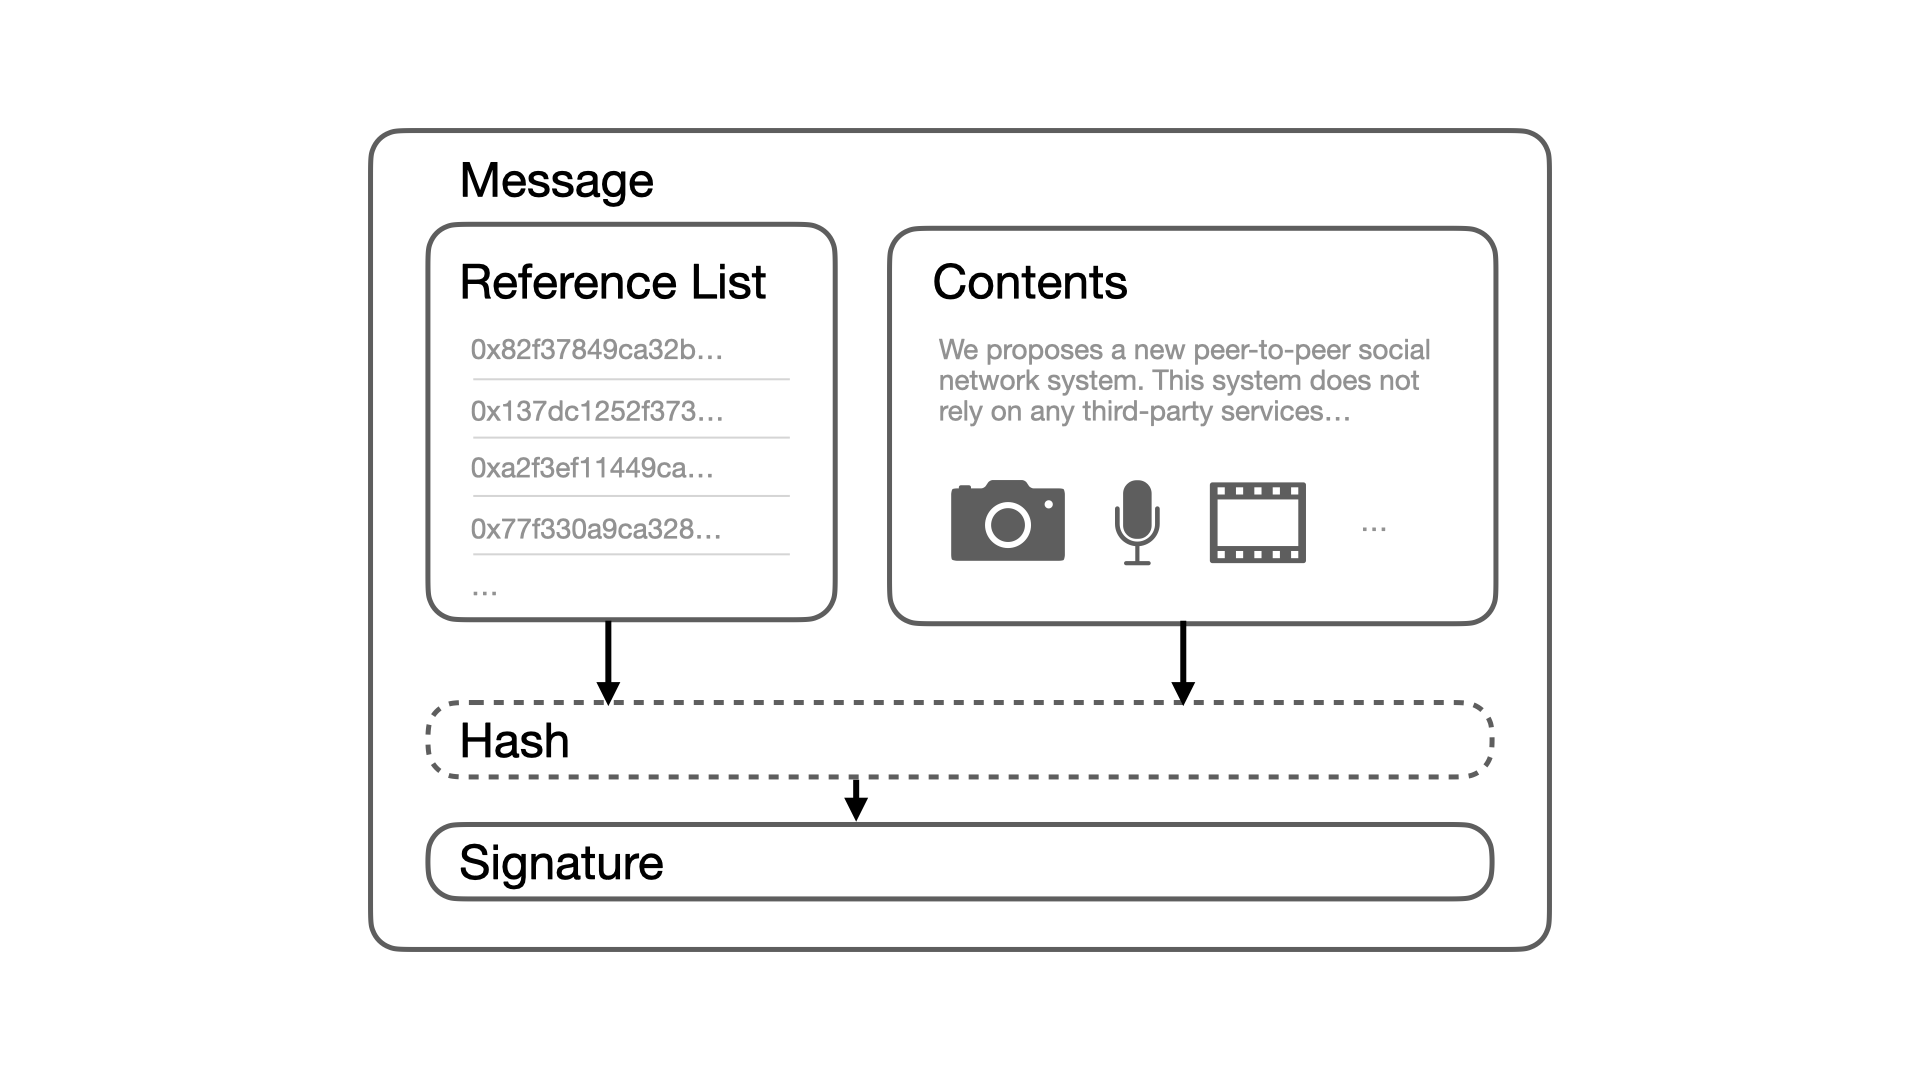
\includegraphics[width=1\linewidth]{message-structure.png}
   \caption{Structure of Message. }
   \label{fig:message}
\end{figure}

As shown in Figure~\ref{fig:message}, each message consists of three parts: message content, a reference list, and a signature. The message content is the main body of the message, divided into content information and interaction types. The former includes multimedia content such as text and images, while the latter encompasses common social network interactions like posting, replying, quoting, and liking. The reference list may contain the signatures of multiple messages, indicating the temporal relationship between the current message and the referenced messages. When the message content involves interactions like replies or quotes, the signatures of the related messages should also be included in the reference list. For more precise temporal verification, it is recommended to include at least one signature of the most recent message in the reference list. Finally, the message content and reference list are merged to calculate a hash value, which is signed using the current publisher’s private key to confirm the publisher's identity and ensure data integrity.

Although each message has explicit content, it is often impossible to determine if a message is spam based solely on the message itself. For instance, messages like "Recommend trying restaurant A on M Street" or "Advise everyone to avoid restaurant B on N Street" might seem fine individually. However, if thousands of similar messages appear in a short time, they are deemed spam and malicious manipulation. In centralized platforms, all user actions are recorded by the platform. Even if users delete their content afterward, the platform's algorithms capture the malicious content and restrict or ban the accounts that posted it, ensuring that malicious behavior is punished and legitimate content is not overwhelmed.

Therefore, a method is needed to access all information posted by an account when necessary and ensure that the posted content has not been tampered with. This helps in evaluating the publisher to determine whether their content is legitimate and if they need to be blocked to reduce spam. Additionally, an effective publisher filtering mechanism is required to ensure that malicious publishers cannot simply switch private keys to continue their behavior after being penalized.

\section{Publisher}\label{sec:publisher}

To accurately assess accounts, we need to ensure that the content published by the accounts has not been tampered with and can be detected even if the publisher deletes the messages. In a peer-to-peer distributed system, this feature is implemented by requiring the content published by each account to form a blockchain-like linked list structure~\cite{Bitcoin}. It is stipulated that the first entry in the reference list of each message must be the signature of the previous message signed by the same private key, as shown in Figure~\ref{fig:publisher}. If the current message is the first message signed by this private key, the first value in the reference list is 0, indicating the starting point.


\begin{figure}
   \centering
   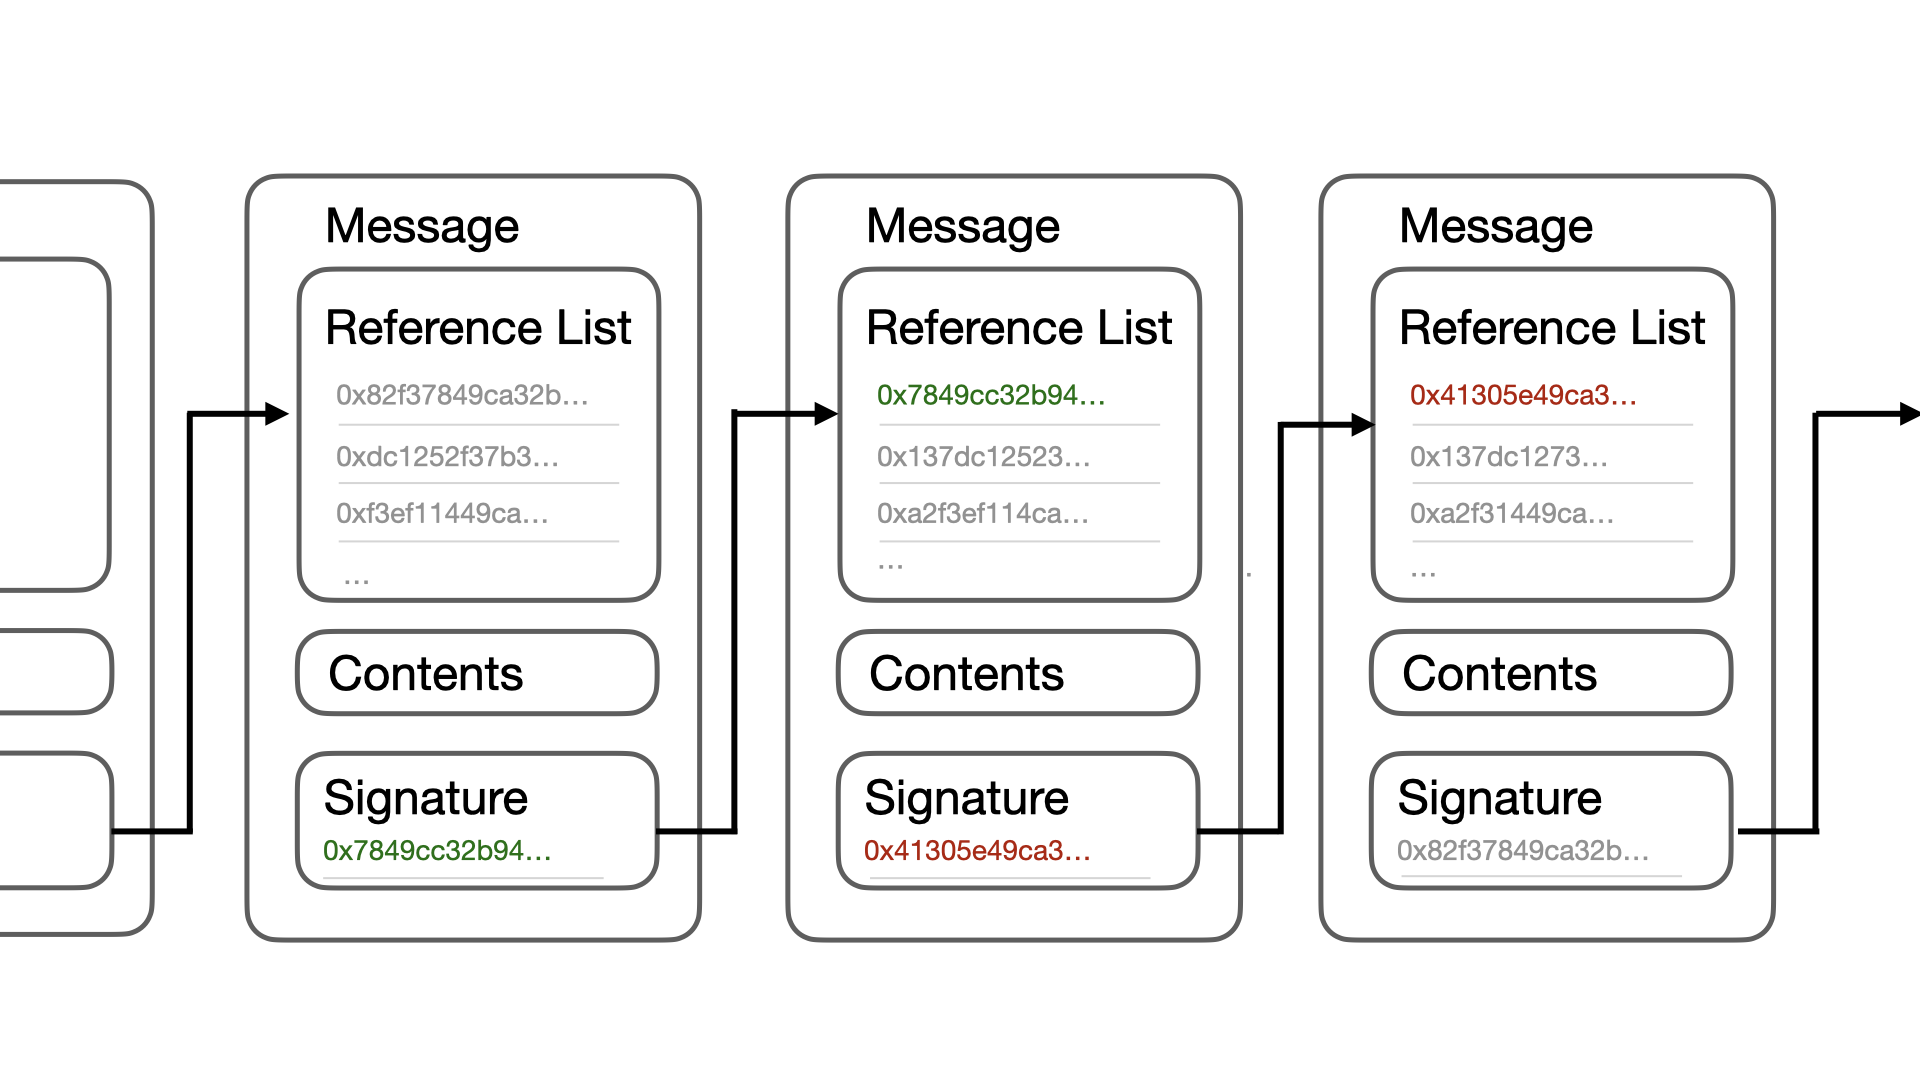
\includegraphics[width=1\linewidth]{publisher_id.png}
   \caption{The sequence of messages signed by the same private key constitutes the publisher. }
   \label{fig:publisher}
\end{figure}

In blockchain systems, forks in the main chain occur due to computational competition among miners rather than malicious behavior. Therefore, the system does not penalize miners for forks but instead achieves consensus through a consensus mechanism. In this system, since signatures cannot be forged, if a publisher's message linked list forks, it is considered intentional modification of historical data by the publisher, which is subjective malicious behavior. Except for the first message, if the first signature in the reference list points to a message signed by a different private key, it is also considered subjective malicious behavior. In both cases, the publisher should be penalized.

If the first message in the reference list has not yet been received, the message should be temporarily stored, and neither trusted nor the publisher penalized. The publisher is responsible for maintaining a complete message chain signed by themselves to provide verification in case any message is lost in the network.

Another scenario is where the publisher may hide a forked message chain, waiting until multiple messages in one fork have been received before publishing messages from another fork into the system. In such cases, the already accepted messages in the system will be considered established facts. Punishment for the publisher typically involves discarding the later-received messages in the conflicting part and blocking the publisher. This punitive approach renders fork attacks meaningless.
\section{Visible Identity Set}\label{sec:visible-identity-set}

In a publisher identity system based on message chains signed by the same private key, other participants can easily assess the credibility of an identity and whether it publishes spam, thereby deciding to block it. However, if an identity is blocked, malicious actors can change their signing private key at no cost and continue publishing messages, rendering the punishment mechanism ineffective.

Traditional centralized platforms usually require phone number verification or similar methods to link a user's real identity to the creation of a virtual identity. Some decentralized identity systems, like Sovrin and Civic, employ similar methods, which are relatively reasonable but rely on trusted third-party verification. Some blockchain-based social systems impose a token cost for account creation. However, given the varying wealth conditions of users, it is challenging to find a price that can attract users while suppressing the creation of spam accounts.

In a decentralized social network, we need a limited and variable set of publisher identities. This set can vary for each system user, eliminating the need for uniform rules to define the identity set. In a peer-to-peer distributed system, all information is based on public messages. These messages already include interactions such as comments and likes. From any publisher identity's message chain, we can calculate which publishers they have interacted with and generate multiple identity sets based on different interaction behaviors. These sets can be combined through various set operations to yield different results. For identities in the resultant set, we can further search for publishers who have interacted with them, gradually expanding the number of identities in the visible user set.

It is important to note that the visible identity set is not equivalent to followers on traditional centralized platforms but is more akin to all users on a traditional platform. Only the information published by identities within this scope can be seen by the user. This visible user set can be directly expanded by the user or automatically expanded or reduced according to defined rules. For instance, if a user in the set interacts with another user, the passive party’s identity can be added to the visible identity set. Conversely, if an identity is deemed a spammer, the identity that introduced this spammer to the visible identity set can also be blocked.

When establishing the visible identity set, if the user has one or more publisher identities, these identities can serve as the starting point for expanding the visible set. However, these identities have no essential difference from other identities in the expansion process. There is no binding relationship between a publisher identity and the visible user set.

The visible user set can be considered a custom rule by which users gradually compute their visible user range based on public information. In a peer-to-peer distributed system, the system does not guarantee users access to all information. Hence, even when using the same rules, the final visible identity sets may differ.

Due to the existence of the visible user set, malicious publishers can change private keys and publish information under a new identity at no cost. However, the new publisher identity will not easily be accepted by other users, reducing the spread of spam and its impact on system users. Even if an identity does not publish spam, frequent interactions with punished publishers may lead to its removal from the visible user set by users.

\section{Network}\label{sec:network}

A decentralized network comprises numerous nodes, each generating a relatively fixed hash value for identification. Nodes filter received messages based on their customized visible identity sets. There is no binding relationship between the information publisher and the node address, nor are they restricted by the visible identity set. Publishers can interact with any message, regardless of the node or publisher from which the messages originated. Whether a new message is accepted by a node depends solely on whether the message's publisher is within the node's visible identity set, independent of the original message.

When an identity is accepted by only a few nodes in the network, due to the peer-to-peer message transmission method, many nodes that accept the identity may still be unable to receive new messages because of other nodes' filters. In this scenario, the spread of information is limited, and the message's impact might be minimal. However, through interactive messages such as comments, forwards, references, and likes, the message's reach can be indirectly expanded. High-quality messages often manage to extend their influence and reach through these interactions, leading to broader acceptance by more nodes.

This propagation mechanism helps balance and optimize information dissemination. Although some messages may have a limited initial spread, high-quality content can overcome these initial restrictions through various forms of interaction within the network, expanding its reach and eventually disseminating more widely among nodes.

\section{Incentives}\label{sec:incentives}

In a social network, the measure of a publisher's self-interest lies in the extent of their information dissemination. The primary objective of a publisher can be considered to maximize the spread of their information. Therefore, in this peer-to-peer distributed network, incentives for publishers are reflected in aiding the expansion of their information dissemination, while penalties are aimed at reducing it. Unlike decentralized systems represented by blockchains, social networks do not have a system-wide consensus, and thus, there are no unified incentives or penalties for a publisher's identity. Incentive mechanisms are based on the statistical outcomes of all information recipients' behaviors.

When a publisher consistently produces high-quality content, their content is more likely to interact with other publishers. Through these interactive messages, the current publisher's content is more likely to be accepted by nodes that have not yet included the current publisher's identity in their visible identity set. As more nodes accept their identity, the number of nodes that can directly receive their messages increases when they broadcast them. This process allows the content of the current publisher to gain an increasingly wider reach over time.

Conversely, if a publisher consistently posts spam or frequently interacts with spam messages, other publishers will be less inclined to interact with them. Some nodes that have already accepted the current publisher's identity may remove this address from their visible user set. Thus, the behavior and content quality of a publisher directly affect the reach and impact of their information. Here, spam refers not only to messages containing explicit content, violence, or hate speech but also to a large volume of meaningless or repetitive information.

In summary, the incentive mechanism of a social network forms a dynamic balance of information dissemination through feedback on the behavior and content quality of publishers. High-quality content publishers can expand their information dissemination and influence, ultimately monetizing their influence through interactions with commercial brands. This process is similar to the advertising system on centralized platforms, encouraging publishers to continuously optimize their content quality to achieve broader dissemination and greater economic benefits.

\section{Blockchain}\label{sec:blockchain}

In the current system, blockchain-based cryptocurrencies can be directly implemented. A block from the blockchain can be encapsulated into a message format, broadcasted by miners as information publishers.

Unlike traditional blockchains, publisher identities in a social system already hold significance. Therefore, more efficient consensus mechanisms can be selected without solely relying on computational power. The system can utilize publisher identities as substitutes for staking, limiting the scope of miners or validators. This approach avoids expanding a publisher's acceptance through successful block production, thereby maintaining the current system's incentive principles. Consensus mechanisms such as Proof of Stake (PoS), Delegated Proof of Stake (DPoS), Proof of Authority (PoA), and Avalanche are suitable choices.

The implementation of cryptocurrency can also be seen as a higher-level publisher composed of multiple publishers. The blockchain, involving these publishers, forms a higher-level total order message queue. The blockchain implemented within the system can identify the total order of block messages through specific positions in the reference list.

\section{Privacy}\label{sec:privacy}

In traditional centralized social networks, privacy protection is achieved by setting different access permissions for users. However, in decentralized social networks, users need to define their identities based on public messages, requiring all public messages to be complete and totally ordered. If a user chooses to encrypt a message before broadcasting it, other users who cannot decrypt it will see it as meaningless spam and will be unable to interact with it, thereby affecting the acceptance of the publisher's identity. Consequently, the incentive mechanism in the current system encourages all publishers to share open and transparent information.

For communications with access restrictions similar to those in traditional social networks, such as one-to-one or one-to-many interactions, privacy can be protected by encrypting the content with the recipient's public key. This method leverages the publisher identities within the current network for peer-to-peer encrypted communication. However, it is important to note that this type of privacy-protected message exchange does not belong to the current peer-to-peer social system. The system's message format should be avoided to prevent erroneous penalties.

Although the information in the system is public, publishers can choose to keep their public keys anonymous. In this scenario, the public can see the content of the messages but cannot associate the publisher's identity in the network with their real-world identity. This method of blocking information flow can also be used to protect privacy.

\section{Third-Party Services}\label{sec:third-party-services}

As a peer-to-peer social network system, we welcome the presence of third-party services but do not rely on any of them. Third-party services can leverage the public messages within the system to provide users with more efficient and convenient services and offer richer ways to interact outside the system.


\begin{description}
   \item[Information Retrieval] Provides message retrieval interfaces based on public messages, with as broad a visible user range as possible.
   
   \item[Message Transmission] Offers peer-to-peer encrypted message transmission services between users based on publisher identities.
   
   \item[Data Analytics] Analyzes public messages and publisher identities to track interaction statistics and calculate the degree of information dissemination.
   
   \item[Advertising Platform] Connects publishers with advertisers based on publisher identities and the extent of information dissemination.
   
   \item[Other Services] Since publisher identities incur a cost, additional services such as voting can be implemented.
   
\end{description}

\section{Conclusions}

We have proposed a peer-to-peer social network system that operates without relying on any third-party services. First, we defined a unified message format where messages signed by the same private key and having a total order constitute the publisher's identity. However, if new users can create identities at zero cost, identity-based penalties will fail to effectively filter spam. To address this issue, we allow information recipients to generate visible identity sets based on the interaction relationships between messages, using customizable rules. Unlike traditional centralized social networks, the filtered messages in this system do not possess system-wide consistency.

The visibility of publishers arises from the interactions between messages. High-quality content publishers attract interactions from other publishers, which, through the spread of interactive messages, further expand the acceptance of their identity. This incentive mechanism encourages publishers to continuously create valuable content.

While all messages in the system are public, users can still transmit encrypted data through other means based on established identity information. Additionally, by blocking information, users can separate network identities from real-world identities, further protecting privacy.

This system can easily integrate existing mainstream blockchain consensus mechanisms. Given the cost of identity creation within the system, it simplifies the implementation of some consensus mechanisms that require staking. This design not only enhances the security and stability of the system but also optimizes the user experience, making decentralized social networks more feasible and attractive.



% 3rd-party clients allow bsky pbc to offer a more curated, opinionated service with stronger moderation, protecting bsky brand
% e.g. bsky own labelers mandatory
% clients may bundle moderation defaults, e.g. enforcing usage of a particular labeler
% can't ban 3rd-party clients like reddit apollo
% prior art: content that is illegal e.g. in germany: twitter filters it out client-side

% Do we want to talk about some kind of robots.txt-like mechanism through which users can specify preferences regarding crawling and indexing?

% Do we want to include some sort of discussion about business models? How do the operators of app views, labelers, etc. get paid?

% \begin{acks}
% \end{acks}

\bibliographystyle{ACM-Reference-Format}
%%% -*-BibTeX-*-
%%% Do NOT edit. File created by BibTeX with style
%%% ACM-Reference-Format-Journals [18-Jan-2012].

\begin{thebibliography}{11}

%%% ====================================================================
%%% NOTE TO THE USER: you can override these defaults by providing
%%% customized versions of any of these macros before the \bibliography
%%% command.  Each of them MUST provide its own final punctuation,
%%% except for \shownote{}, \showDOI{}, and \showURL{}.  The latter two
%%% do not use final punctuation, in order to avoid confusing it with
%%% the Web address.
%%%
%%% To suppress output of a particular field, define its macro to expand
%%% to an empty string, or better, \unskip, like this:
%%%
%%% \newcommand{\showDOI}[1]{\unskip}   % LaTeX syntax
%%%
%%% \def \showDOI #1{\unskip}           % plain TeX syntax
%%%
%%% ====================================================================

\ifx \showCODEN    \undefined \def \showCODEN     #1{\unskip}     \fi
\ifx \showDOI      \undefined \def \showDOI       #1{#1}\fi
\ifx \showISBNx    \undefined \def \showISBNx     #1{\unskip}     \fi
\ifx \showISBNxiii \undefined \def \showISBNxiii  #1{\unskip}     \fi
\ifx \showISSN     \undefined \def \showISSN      #1{\unskip}     \fi
\ifx \showLCCN     \undefined \def \showLCCN      #1{\unskip}     \fi
\ifx \shownote     \undefined \def \shownote      #1{#1}          \fi
\ifx \showarticletitle \undefined \def \showarticletitle #1{#1}   \fi
\ifx \showURL      \undefined \def \showURL       {\relax}        \fi
% The following commands are used for tagged output and should be
% invisible to TeX
\providecommand\bibfield[2]{#2}
\providecommand\bibinfo[2]{#2}
\providecommand\natexlab[1]{#1}
\providecommand\showeprint[2][]{arXiv:#2}

\bibitem[\protect\citeauthoryear{Hatamleh, Safori, Habes, Tahat, Ahmad, Abdallah, and Aissani}{Hatamleh et~al\mbox{.}}{2023}]%%
{Trust}
\bibfield{author}{\bibinfo{person}{Hatamleh, I.H.M.}, \bibinfo{person}{Safori, A.O.}, \bibinfo{person}{Habes, M.}, \bibinfo{person}{Tahat, O.}, \bibinfo{person}{Ahmad, A.K.}, \bibinfo{person}{Abdallah, R.A.-Q.}, \bibinfo{person}{Aissani, R.}} 
\bibinfo{year}{2023}\natexlab{}.
\newblock \bibinfo{title}{Trust in Social Media: Enhancing Social Relationships}.
\newblock
\newblock
\urldef\tempurl%
\url{https://www.mdpi.com/2076-0760/12/7/416}
\showURL{%
\tempurl}

\bibitem[\protect\citeauthoryear{La Cava, Greco, and Tagarelli}{La Cava et~al\mbox{.}}{2021}]%%
{Mastodon}
\bibfield{author}{\bibinfo{person}{La Cava, L.}, \bibinfo{person}{Greco, S.}, \bibinfo{person}{Tagarelli, A.}} 
\bibinfo{year}{2021}\natexlab{}.
\newblock \bibinfo{title}{Understanding the growth of the Fediverse through the lens of Mastodon}.
\newblock
\newblock
\urldef\tempurl%
\url{https://arxiv.org/pdf/2106.15473}
\showURL{%
\tempurl}

\bibitem[\protect\citeauthoryear{Steemit}{Steemit}{2024}]%%
{Steemit}
\bibfield{author}{\bibinfo{person}{Steemit}} 
\bibinfo{year}{2024}\natexlab{}.
\newblock \bibinfo{title}{Steem Platform Whitepaper 2.0}.
\newblock
\newblock
\urldef\tempurl%
\url{https://github.com/steemit/whitepaper}
\showURL{%
\tempurl}

\bibitem[\protect\citeauthoryear{Thelwall}{Thelwall}{2018}]%%
{SteemitModel}
\bibfield{author}{\bibinfo{person}{Thelwall, M.}} 
\bibinfo{year}{2018}\natexlab{}.
\newblock \bibinfo{title}{Can social news websites pay for content and curation? The SteemIt cryptocurrency model}.
\newblock
\newblock
\urldef\tempurl%
\url{https://sci-hub.ru/10.1177/0165551517748290}
\showURL{%
\tempurl}

\bibitem[\protect\citeauthoryear{Ottman and Doe}{Ottman and Doe}{2019}]%%
{Censorship}
\bibfield{author}{\bibinfo{person}{Ottman, B.}, \bibinfo{person}{Doe, J.}} 
\bibinfo{year}{2019}\natexlab{}.
\newblock \bibinfo{title}{The Censorship Effect}.
\newblock
\newblock
\urldef\tempurl%
\url{https://cdn-assets.minds.com/The_Censorship_Effect.pdf}
\showURL{%
\tempurl}

\bibitem[\protect\citeauthoryear{Nakamoto}{Nakamoto}{2008}]%%
{Bitcoin}
\bibfield{author}{\bibinfo{person}{Nakamoto, S.}} 
\bibinfo{year}{2008}\natexlab{}.
\newblock \bibinfo{title}{Bitcoin: A Peer-to-Peer Electronic Cash System}.
\newblock
\newblock
\urldef\tempurl%
\url{https://bitcoin.org/bitcoin.pdf}
\showURL{%
\tempurl}

\bibitem[\protect\citeauthoryear{Reed and Hardman}{Reed and Hardman}{2018}]%%
{Sovrin}
\bibfield{author}{\bibinfo{person}{Reed, D.}, \bibinfo{person}{Hardman, D.}} 
\bibinfo{year}{2018}\natexlab{}.
\newblock \bibinfo{title}{How DIDs, Keys, Credentials, and Agents Work Together in Sovrin}.
\newblock
\newblock
\urldef\tempurl%
\url{https://sovrin.org/wp-content/uploads/2019/01/How-DIDs-Keys-Credentials-and-Agents-Work-Together-in-Sovrin-131118.pdf}
\showURL{%
\tempurl}

\bibitem[\protect\citeauthoryear{Jethava and Rao}{Jethava and Rao}{2022}]%%
{TrustEvaluation}
\bibfield{author}{\bibinfo{person}{Jethava, G.}, \bibinfo{person}{Rao, U.P.}} 
\bibinfo{year}{2022}\natexlab{}.
\newblock \bibinfo{title}{An Interaction-Based and Graph-Based Hybrid Approach to Evaluate Trust in Online Social Networks (OSNs)}.
\newblock
\newblock
\urldef\tempurl%
\url{https://link.springer.com/article/10.1007/s13369-021-06332-w}
\showURL{%
\tempurl}

\bibitem[\protect\citeauthoryear{Lin, Gao, and Li}{Lin et~al\mbox{.}}{2020}]%%
{Guardian}
\bibfield{author}{\bibinfo{person}{Lin, W.}, \bibinfo{person}{Gao, Z.}, \bibinfo{person}{Li, B.}} 
\bibinfo{year}{2020}\natexlab{}.
\newblock \bibinfo{title}{Guardian: Evaluating Trust in Online Social Networks with Graph Convolutional Networks}.
\newblock
\newblock
\urldef\tempurl%
\url{https://ieeexplore.ieee.org/abstract/document/9155370}
\showURL{%
\tempurl}

\bibitem[\protect\citeauthoryear{Khaksari and Keyvanpour}{Khaksari and Keyvanpour}{2019}]%%
{TrustPrediction}
\bibfield{author}{\bibinfo{person}{Khaksari, A.}, \bibinfo{person}{Keyvanpour, M.R.}} 
\bibinfo{year}{2019}\natexlab{}.
\newblock \bibinfo{title}{TP-TA: A Comparative Analytical Framework for Trust Prediction Models in Online Social Networks Based on Trust Aspects}.
\newblock
\newblock
\urldef\tempurl%
\url{https://link.springer.com/article/10.1007/s10462-017-9583-1}
\showURL{%
\tempurl}

\bibitem[\protect\citeauthoryear{Ureña, Kou, Dong, Chiclana, and Herrera-Viedma}{Ureña et~al\mbox{.}}{2019}]%%
{TrustPropagation}
\bibfield{author}{\bibinfo{person}{Ureña, R.}, \bibinfo{person}{Kou, G.}, \bibinfo{person}{Dong, Y.}, \bibinfo{person}{Chiclana, F.}, \bibinfo{person}{Herrera-Viedma, E.}} 
\bibinfo{year}{2019}\natexlab{}.
\newblock \bibinfo{title}{A Review on Trust Propagation and Opinion Dynamics in Social Networks and Group Decision Making Frameworks}.
\newblock
\newblock
\urldef\tempurl%
\url{https://www.researchgate.net/publication/329039753_A_review_on_trust_propagation_and_opinion_dynamics_in_social_networks_and_group_decision_making_frameworks}
\showURL{%
\tempurl}


\end{thebibliography}
\end{document}
